\chapter{Distributed analysis with GROSS}

\section{Introduction}
GROSS (GRidified Orca Submission System)~\cite{CHEP04_TALLINI} was created to provide a reliable method for submitting CMS analysis jobs to experiment resources worldwide. It was designed to perform all of the major operations required by physicists when submitting large analysis tasks, i.e. once the analysis code had been developed and an analysis of large amounts of data was required. The user's analysis task was split into smaller, independent jobs which were submitted to a batch system. These were monitored and any output retrieved.

%The aim of GROSS was to allow users to submit their analysis jobs to the experiments worldwide resources via the grid. However before DC04 there was virtually no (possibly none at all) user analysis conducted over the grid as there was no policy for distributing event data to the sites. For most analyses both code development and running jobs were carried out at CERN. To increase the chances of users adopting GROSS it was decided that GROSS be able to submit to both grid and local resources.

To guide the design of the CMS Computing Model a series of increasingly complex data challenges were run. One of the major challenges was CMS Data Challenge 2004 (DC04)~\cite{citeulike:876074}. A principal aim of this challenge was to perform distributed analysis, and it was this role that GROSS was designed to fill. At the time users generally used local batch resources therefore it was decided that GROSS should submit to both grid and local resources. 

\section{CMS Data Challenge 2004}
The main components of the challenge were:
\begin{itemize}
\item{Event reconstruction at the Tier-0 at a rate of 25Hz for 1 month;}
\item{Transfer of the RAW and reconstructed data to Tier-1 and Tier-2 sites; and}
\item{Analysis at remote sites.}
\end{itemize}
%To take the place of the CMS detector an online process made pre-generated CMS event data available to the reconstruction system at a rate of 40 MB/s. 
Prior to DC04 70 million Monte Carlo events had been prepared and moved to the CERN Tier-0. These events were fed to the reconstruction farm, comprising $\sim$500 CPUs, at a rate of 40 MB/s. The reconstructed output from this farm, at a data rate of $\sim$4 MB/s, was stored at the Tier-0. Both the RAW and RECO data were then copied from the Tier-0 to remote sites where analysis jobs were run.

%Prior to this challenge it was realised that there was no tool that could perform distributed analysis: either for DC04 or the end user. Hence it was decided to develop GROSS to fill this gap.

%\section{CMS offline computing during DC04}
At the time of DC04 most of the components listed in the computing model did not exist. It was during this time that the forerunners to these systems were developed. 

\subsection{CMS analysis framework}
The forerunner to the current CMS analysis framework was called ORCA (Object-oriented Reconstruction for CMS Analysis)~\cite{citeulike:876402}. The ORCA framework was based on POOL but was limited to accessing local data, which restricted users to a small subset of the available computational and storage resources. %ORCA required all input files be listed in a POOL file catalogue.

\subsection{Event data model}
The event data model used during DC04 was significantly different to that described in the computing model. RAW data was split into two data tiers called Hits and ``Digis'', following the GEANT terminology~\cite{geant}. The Hits, only available for Monte Carlo data, contained the simulated physics process and held the Monte Carlo truth while Digis held the digitised detector response. Most analyses, at the time, required both the detector response and Monte Carlo truth and so required both data tiers. A new label, the owner name, contained both the data tier and software versions used. When specifying data for analysis both the dataset and owner name were required. For the remainder of the chapter, unless otherwise stated, the term ``dataset'' refers to the unique dataset/owner pairing. 

%The data tier (HIT, DIGI) was represented in a different field, the owner name, along with the software version used. 

CMS data were split into two file types: event and metadata. The event data contained the actual events while the metadata indexed the collections held within the event files. When ORCA required a certain event within a dataset it would look in the metadata to find a pointer to the relevant file and event collection. When the specification for a Monte Carlo dataset was created, so was the metadata, and this was referred to as ``virgin'' metadata. Each run within the dataset was generated separately against the virgin metadata. Once all of the runs had been finished, the virgin metadata files were populated with information about all runs, a process which required access to all files. This ``final'' metadata knew about all event collections within the dataset and allowed an analysis to proceed.

Due to an unfortunate naming convention, datasets with the same owner name, i.e. data tier and software version, all had metadata files with the same name. This, and the need for simultaneous access to all event data to populate the metadata, complicated their registration to the RLS. As a temporary measure during DC04 the virgin metadata files were placed into an archive that was registered with the RLS. ORCA could run on the virgin metadata if the ORCA configuration file explicitly listed the event collections to be used.

\subsection{CMS software available at sites}
Due to the large size of ORCA and its dependencies (more than 600 MB) it was decided that each site would have a centrally-installed copy. A job needed only to carry its executable and private libraries with it and could rely on a pre-installed version of all standard ORCA libraries to be available. For each version of ORCA installed a tag was added to the information published by the site in the grid information system. When a job was submitted this allowed the RB to locate all sites with the required software and thus steer the job to an appropriate location.

\subsection{Data replication and discovery}
Data movement was managed by a group of semi-autonomous software agents collaborating through the Transfer Management DataBase (TMDB). This is illustrated in Figure~\ref{fig:data_transfer}~\cite{citeulike:623034, Fanfani:2004gh}. Data was copied from CERN to the sites using standard LCG replication tools. These data were stored on LCG SE's with at least two copies of each file, one located at CERN and one at a Tier-1 site. The files were registered with the RLS. During DC04 the RLS file metadata attributes were used to store information about the event collections contained within the file, these being dataset, owner and run number.

\begin{figure}[tbp]
  \centering
  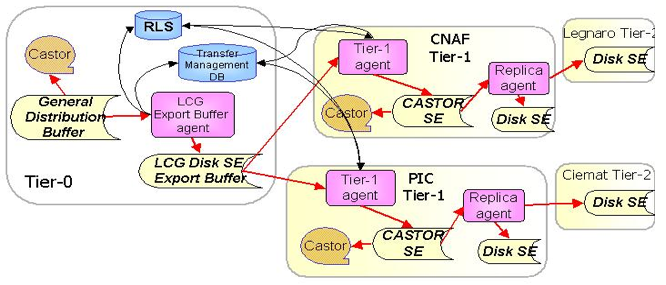
\includegraphics[width=0.95\linewidth]{gross/data_transfer}
  \caption{The DC04 data distribution system.~\cite{Fanfani:2004gh}
  \label{fig:data_transfer}}
\end{figure}

When preparing analysis jobs data discovery was handled through the RLS. Queries were performed with the POOL file catalogue commands. The list of LFN's returned were then listed in the analysis job JDL. Upon receipt of the job the RB looked at the list of LFN's and used the RLS to find sites that held replicas of the required files. The RB then submitted the job to a site within the list.

\subsection{BOSS}
CMS job tracking and submission at this time was handled by BOSS (Batch Object Submission System)~\cite{citeulike:342741}. BOSS was initially developed as a tool for MC production activities at CMS sites and provided a uniform interface to a variety of batch schedulers. It had no CMS specific concepts and thus required directing by a CMS specific application. For production this was McRunJob~\cite{citeulike:867593} but no similar tool existed for analysis. McRunJob created CMS production jobs and used BOSS for job submission and tracking. The advantages of this were that McRunJob could concentrate on CMS-specific functionality (in particular interfacing with the CMS MC production database, RefDB) with BOSS responsible for all common job actions, such as submission and tracking.

BOSS was not a batch scheduler (the workflow is shown in Figure~\ref{fig:boss_Workflow}) and relied on an underlying implementation interfaced via a plugin mechanism. Each batch scheduler was registered to the BOSS system along with a variety of simple wrapper scripts designed to perform standard job actions (submit, query etc.). These were saved to the database with no changes to the core code. When a user requested that BOSS interact with a particular scheduler, the script for the desired action was retrieved and executed. This enabled BOSS to present a uniform interface to multiple schedulers.

\begin{figure}[tbp]
  \centering
  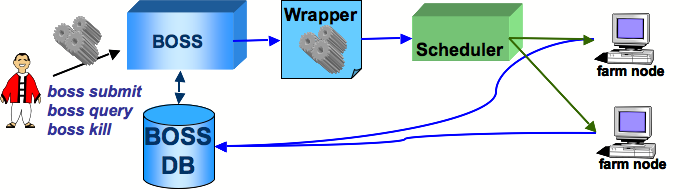
\includegraphics[width=0.95\linewidth]{gross/boss_workflow}
  \caption{The basic BOSS workflow.~\cite{citeulike:342741}
  \label{fig:boss_Workflow}}
\end{figure}

For persistency BOSS used a MySQL database, which was used to store configuration options and job details. Persistent job information stored to the database included details given during job creation such as executable name and input and output files. Once submitted a job returned monitoring information directly to the database. 
%where it was available to the user via the BOSS command line client. 

BOSS also allowed the user to specify the type of executable in the job, called ``job type'', to activate customised monitoring. By registering a job type a user could specify values that were monitored in the application's standard input, output and error streams. This monitoring was performed by a set of scripts, with one for each of the streams that required monitoring. To register a job type the user had to specify a schema that listed the variables to monitor and the set of scripts responsible for monitoring the streams and returning the correct values. For each job type a new table was created in the database with a separate column for each parameter. Each job was represented by a single row and only the last value in each category was retained. When a user specified the job type the relevant scripts were retrieved from the database and sent with the job. This customised monitoring had been used within CMS previously to, for example, record the current event number and allow the job's progress to be monitored. 

User interaction with BOSS was via a Command Line Interface (CLI) or API. The API was a basic C++ API that accepted the same options as the CLI. Simple jobs could be defined by options to the CLI (or API), e.g.. executable name, type and any arguments, while a more complicated job could be described in a Job Description Language (JDL) file. The JDL file was written in the same Classified Advertisement (ClassAd)~\cite{citeulike:835507} syntax as the LCG JDL file. 

Job creation and submission could be combined in a single step or split into two distinct operations. When a job was created BOSS processed the ClassAd file (if used), performed basic checks and saved it to the database. The job was then ready to be submitted. Upon job submission BOSS retrieved the relevant job information from the database and created various submission files. These consisted of files the user requested be sent with the job, the executable and various BOSS programs and files. The BOSS files sent included a job specification file, the monitoring scripts (optional), a program responsible for sending monitoring information back to the database (dbUpdator) and the main BOSS job wrapper (jobExecutor). 

Once the job started the jobExecutor took responsibility for starting the monitoring, running the user's executable and performing cleanup actions. The jobExecutor wrote a log file (journal file) containing a complete log of the job's activity, including general details (start time, execution host, etc.) as well as the information provided by the monitoring scripts. The dbUpdator monitored the journal file and relayed any new information to the database. 

By using the BOSS client the user could query the status of their job. BOSS would first look into the database and, if it was unable to determine the status from this (because for example the job had been submitted but no output had been retrieved) it would query the scheduler.  

When the job finished the output was returned to the user. The output was either saved to a shared filesystem if submitted to a local scheduler or saved to the RB in the case of LCG submission. To obtain output in the LCG case a separate command had to be run. In both cases the output files included the output requested by the user as well as the journal file and the standard output and error. If the dbUpdator was unable to contact the database during execution (generally due to a firewall) then a command could be run that parsed the journal file and populated the database.

%%%%%
%BOSS architecture C++ etc...
%Monitoring need db access. 
%POOL/RLS or in grid chapter?
%API
%May need to expand later - more details when talking about BOSS version 4.
%%%%%

%\section{Overview}
%GROSS was created to provide a reliable method for submitting ORCA jobs to the experiments worldwide resources, for both DC04 and end user analysis. GROSS was designed to handle all the major operations that physicists require when submitting large analysis tasks i.e. once they have written their analysis code and need to run over large amounts of data. GROSS took a users analysis task, split the task into many smaller independent jobs, submitted the jobs to a batch system, monitored them and handled any output files.

%The aim of GROSS was to allow users to submit their analysis jobs to the experiments worldwide resources via the grid. However before DC04 there was virtually no (possibly none at all) user analysis conducted over the grid as there was no policy for distributing event data to the sites. For most analyses both code development and running jobs were carried out at CERN. To increase the chances of users adopting GROSS it was decided that GROSS be able to submit to both grid and local resources.

% In order to run the users analysis as quickly and efficiently as possible the analysis task would be split into many smaller jobs. Each accessing a small subset of the total dataset. This allows for jobs to run at multiple sites, depending on load, and for individual sites to host partial datasets and still be utilised. 

\section{The GROSS design Process}
Before work on GROSS began a full design process was completed. The first step was to determine what functionality and features were required from such a tool. Prior to starting this work an LCG report titled ``Common use cases for a HEP common application layer for analysis'' (HEPCALL II)~\cite{LHC-SC2-20-2002} was published. This document looked at the various types of analyses that would be conducted at the LHC and what software would be needed to facilitate them. Differing scopes of analysis were studied ranging from end user analysis to large-scale managed analyses. Various levels of interactivity were also investigated ranging from fully interactive through to pure batch work.

\begin{figure}[tbp]
  \centering
  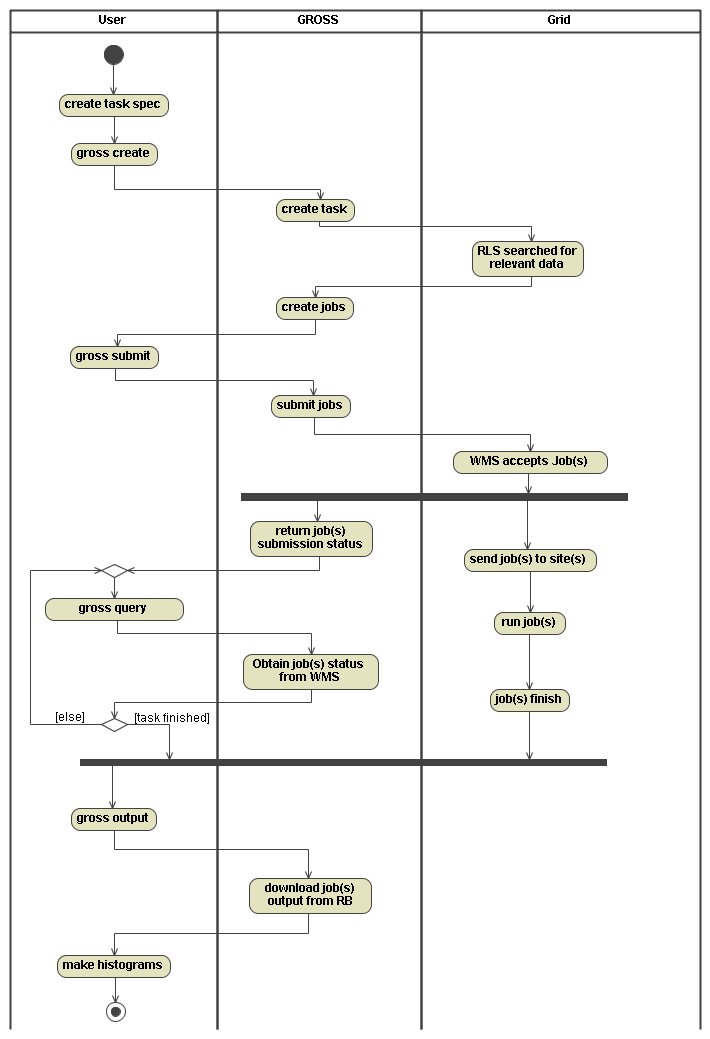
\includegraphics[width=0.95\linewidth]{gross/Overall_Workflow}
  \caption{An activity diagram showing a GROSS workflow consisting of task creation, submission and output retrieval. The User swimlane shows the users actions and the GROSS commands used. The GROSS and Grid swimlanes show the resulting actions of both entities. Note that in this case no output is downloaded until all jobs have competed but this is not compulsory. Output from a job is available for download as soon as the job is finished.
  \label{fig:Overall_Workflow}}
\end{figure}

The end user analyses described in the document included the non-organised analysis r$\acute{e}$gime, where physicists perform un-coordinated work and require as much assistance as possible from the analysis system. The functionality for such a system included file access, job submission and robust provenance mechanisms. The starting point for such an analysis was a query requiring data that met certain criteria (both in terms of data quality and physics attributes), with the user not knowing where the data was located or how to access it. It was also possible that the user had modified parts of the experiments standard analysis code especially for their analysis. The need for logging and provenance information was emphasised with the example of a user attempting to determine where and when certain jobs ran in order to verify their results.

The HEPCAL II document included various models of analyses with varying levels of involvement by the grid WMS in operations such as data discovery and task splitting. The LCG/EGGE did not provide such high levels of functionality and together with the requirement for GROSS to be able to use non-grid resources resulted in GROSS being developed along the lines of the ``No special support by WMS'' model. This resulted in GROSS performing all data discovery, task splitting and job preparation. The WMS treated jobs as simple independent jobs with only a list of site and input data requirements, all features provided by the LCG.

BOSS was a named example of an application with an intermediate level of interactivity where the user had no direct control but did have the ability to monitor closely the process. As GROSS was designed to be used with fully developed analyses interactive control was not required.

From the HEPCAL II description of non-interactive end user analysis with an analysis system designed to work with no special support from the WMS a GROSS use case document was produced. GROSS user requirements were then derived from this document.

The main use case developed for GROSS is illustrated in Figure~\ref{fig:Overall_Workflow}. This workflow described an end user wishing to submit an analysis task and obtain output files. The user had to provide information including ORCA executable, version, configuration file, output file names and the physics data selection query. GROSS would then contact the physics catalogue to discover the list of matching datasets and files. From this GROSS would optionally split the task into multiple jobs, each accessing a subset of the requested data. The task and its sub-jobs would be saved and a numeric identifier (id) returned to the user. With this id the user could then submit the task. Each job was submitted with full monitoring and tracking. At the end of a job the output files would be copied to an SE or brought back with the output sandbox. By running a separate command the user could retrieve the output sandboxes for all jobs in a task.

By the time of DC04 it had become clear that there would be no physics metadata catalogue capable of accepting physics queries and returning a list of matching data. GROSS therefore required the user to specify the requested dataset name when creating the task. If, at a later time, such a physics database was implemented the structure of GROSS would easily allow its use.

Existing tools were utilised whenever possible, minimising duplication of effort and reducing development time. BOSS was used for job tracking, monitoring and submission. Basing GROSS on BOSS allowed GROSS to take advantage of the extensive bookkeeping and job submission features provided within BOSS. GROSS provided the user interface and functionality specific to CMS analysis. 
%GROSS needed a way to contact the RLS and store the returned file list. ORCA required such a list in a POOL file catalogue, therefore it was decided to use this for GROSSs internal file catalogue as well.

\section{Architecture}
One of the main design requirements for GROSS was that it be as modular and flexible as possible. Figure~\ref{fig:Orca_Overview} shows the main GROSS functions and how they relate with external entities. Internally the different components interacted through well-defined interfaces that isolated the rest of GROSS from any component changes. During development the POOL file catalogue API underwent a number revisions but the structure of GROSS restricted the impact of these changes to one component.

GROSS was written in fully object-oriented C++ and utilised design patterns where appropriate. Design patterns are general repeatable solutions to commonly occurring problems within computer science~\cite{citeulike:115158}. 

\begin{figure}[!tbp]
  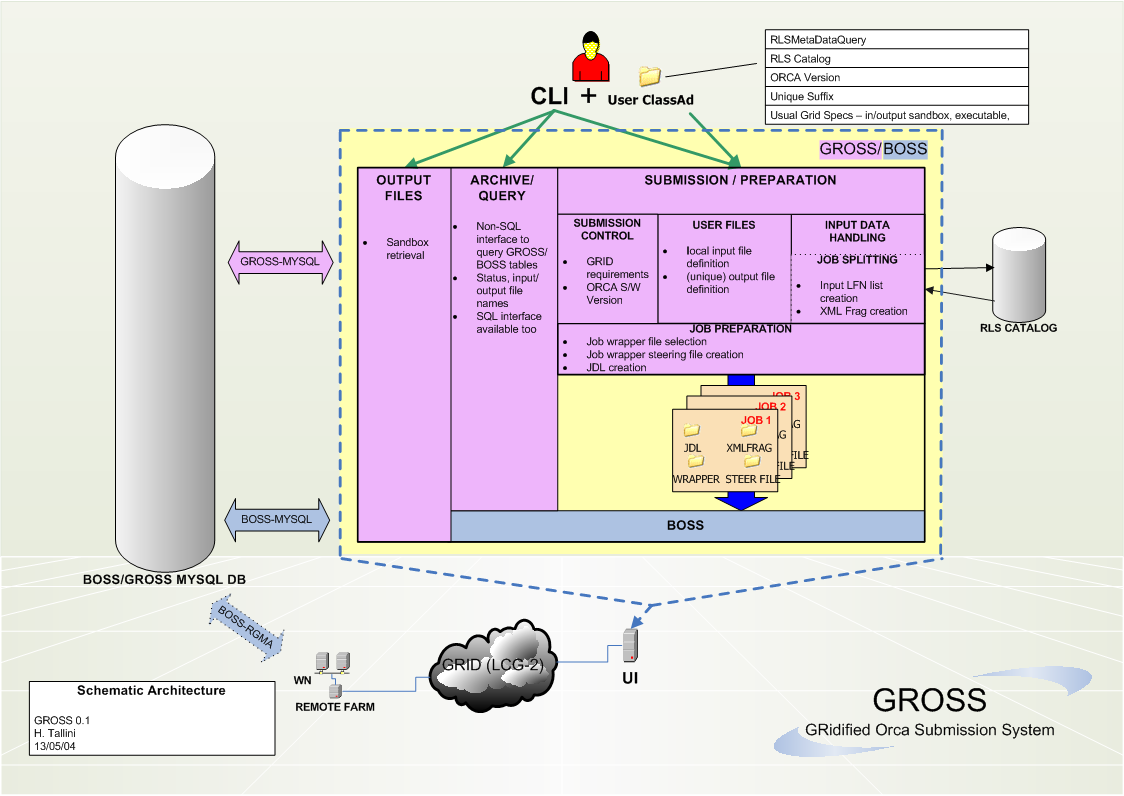
\includegraphics[width=1.5\linewidth,angle=90]{gross/GROSS_Overview_RLS}
  \caption{The main features of GROSS and their relation with external entities.~\cite{CHEP04_TALLINI}
  \label{fig:Orca_Overview}}
\end{figure}

Despite designing GROSS with the primary purpose of creating and submitting ORCA analysis jobs it was decided that GROSS should also be capable of submitting any type of application. Any application-specific functionality had to be part of a modular system. This allowed the future possibility of handling different types of CMS applications, e.g. Monte Carlo production and fast simulation. This was achieved by use of the ``Abstract Factory'' design pattern~\cite{citeulike:115158}, which provides a mechanism for instantiating a family of classes in a uniform and consistent manner. A different family was needed for each supported application (called task types by GROSS). The family provided functionality suited to the particular application including task splitting and submission file preparation.

As BOSS masked the differences between schedulers it had been the original aim that GROSS would remain independent of any scheduler choice, leaving the user free to choose at the time of task submission. However, the large differences in both the execution environment and data access model between grid and non-grid resources made complicated this. A different task type therefore had to be used for ORCA jobs submitted to the grid compared to jobs submitted to a local scheduler. These differences may have been hidden by a sufficiently high abstraction, however this would result in such widely varying requirements for the two cases so as to make it impractical. It was decided that the benefit to the user was outweighed by the development work required, as generally users know if they are submitting to local or remote resources.

The family responsible for ORCA grid jobs is shown in Figure~\ref{fig:OrcaG_Factory}. On the left is the abstract factory that is responsible for instantiating the required classes. When creating a task the type was specified on the command line and the relevant factory implementation instantiated all classes in the family. The task type was saved to the database along with the task so that correct classes could be correctly instantiated in further operations. The family was composed of classes responsible for the task, the jobs, wrapper steering file and JDL. There were two concrete classes responsible for tasks and jobs, one responsible for creating the object from the users specification and the other for retrieving information from the database.

\begin{figure}[!tbp]
  \centering
  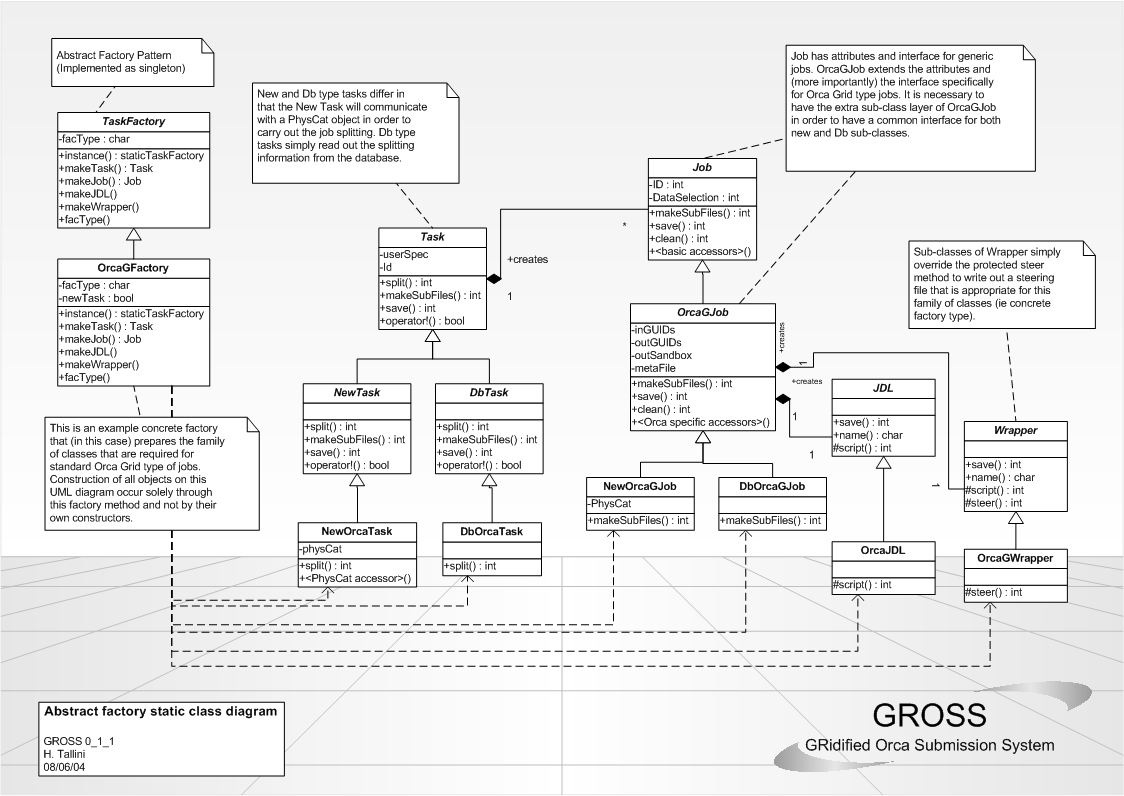
\includegraphics[width=1.4\linewidth,angle=90]{gross/GROSS_UML}\\[1mm]
  \caption{Class diagram showing the abstract factory. ``OrcaG'' refers to the classes responsible for ORCA tasks that are submitted to LCG.~\cite{citeulike:878837}
  \label{fig:OrcaG_Factory}}
\end{figure}

%Database schema - i.e same as BOSS but with a few extra tables.

As GROSS was closely coupled with BOSS it was decided to distribute them together. A user only needed one package and both were installed and configured simultaneously.

As in BOSS it was decided to store all GROSS task information into a database. As most job information was stored into the BOSS database only a few extra tables were required. Thus it was decided to add the GROSS tables to the BOSS database. GROSS access to this database was handled through a singleton~\cite{citeulike:115158}. A singleton is a class that can only be instantiated once, resulting in only one database connection for the whole session. Database calls from all GROSS classes were routed through this object to minimise the database load.

\section{Functionality and interface}
The user interacted with GROSS through a command line client. Options were passed on the command line with the task specification passed via a file (the task specification file). As both BOSS and LCG used ClassAds for their configuration information it was decided to utilise these in GROSS. This allowed GROSS to take advantage of a mature parser library and gave the user a familiar configuration syntax. An added advantage was that unknown fields in the configuration file could be passed down to BOSS, where they might be understood, or, if not, down further to the scheduler. This provided a mechanism for users to provide configuration options direct to the LCG scheduler.

%The GROSS command line took various options depending on whether the user wished to create, submit or monitor a task. All Operations could be performed on a whole task or on a range of jobs within a task. All commands accepted standard parameters that modified the output logging verbosity and BOSS configuration location from their defaults.

\subsection{Task Creation}
%%%%%
%During GROSS's design phase it had been assumed that CMS would have a physcis metadata catalogue that would return data (either dataset or files) that matched a physics query. However by the time of DC04 this catalogue did not exist. Thus a user had to know the name of the dataset they wished to analyse.
%%%%%

Task creation required command line options including task type and the specification file. This file listed all information needed to create the task including the executable file, paths to any libraries required by the application, ORCA version, ORCA configuration file path, the dataset name and output file name. As well as a unique id each task had the option of having a user-defined name associated with it. This was appended to output filenames to aid recognition.

%During task creation the POOL catalogue functionality was used to confirm that the dataset existed and perform the task splitting. Each sub job was configured with the correct data selection, input and output data files. Submission files were generated at this point to allow the user the option of inspecting them before submission. All necessary information was saved to the database, so on subsequent actions the entire task and all jobs could be recreated without repeating the data discovery or task splitting.

\subsection{Input data handling}
At the time of DC04 the expected minimum necessary information required for data discovery was a dataset name. From this GROSS had to be able to discover all data files in the dataset. To allow refinement of this, it was also possible for a user to reduce the scope of the analysis with a further query on the RLS metadata, i.e. on the run number.
%GROSS required an interface to the POOL API that presented all the necessary functionality in a simple and appropriate form.

The ability of the POOL file catalogue to use multiple backend technologies allowed a user to switch between the official CMS RLS and a private POOL file catalogue by changing the file catalogue contact string in the task specification file.

POOL had many dependencies including SEAL~\cite{SEAL} (another LCG project), XML (if used with XML catalogues), MySQL (if used with MySQL catalogues) and BOOST~\cite{BOOST} (a set of C++ libraries). GROSS therefore shared these dependencies. These dependancies would normally have been unacceptable but it was assumed that ORCA, which also required POOL, would be installed to allow the user to develop their analysis. 

Due to the predicted load from the whole collaboration it was decided to reduce the number of queries to the RLS originating from GROSS as much as possible. To accomplish this GROSS implemented a local cache of the relevant information in the RLS. The POOL API provided functionality to extract information from one catalogue and store it in another. Thus the first file catalogue operation performed by GROSS queried the RLS for all information belonging to a dataset and saved this information to a local XML catalogue. All further file catalogue queries were performed on this local copy that, as well as reducing load on the RLS, also improved performance.

%To perform the file catalogue export first a local file catalogue with the same schema as the original had to be created. This involved contacting the existing catalogue, extracting the metadata schema and creating a new local catalogue with the same metadata schema. Then the source catalogue was queried for the owner/dataset pair given by the user and the results saved to the destination catalogue.

One major limitation of the POOL file catalogue API was a lack of ``OR'' logic in query terms; query terms could only be joined with ``AND'' logic or wildcards. GROSS required this functionality for the users optional metadata query, which typically involved queries containing a list of run numbers. To implement this the GROSS POOL interface contained functionality that parsed all query strings for the ``OR'' token. If found the query was split at this point. Each query was then executed separately with the final result set formed from the sum of all partial result sets. Thus, from the user's perspective, ``OR'' functionality was natively supported.

%GROSS made queries of LFN, PFN and run number results from arbitrary complex search queries. The LFN and PFN methods simply queried the catalogue, cycled through the appropriate file name container provided by the API, aggregated the results and returned them. The method that returned the run numbers for the files returned by a query - cycled through a metadata container, provided by the API, searched for the run field and returned a numerically sorted, and unique, list of results to the caller.

%exceptions

\begin{figure}[!tbp]
  \centering
  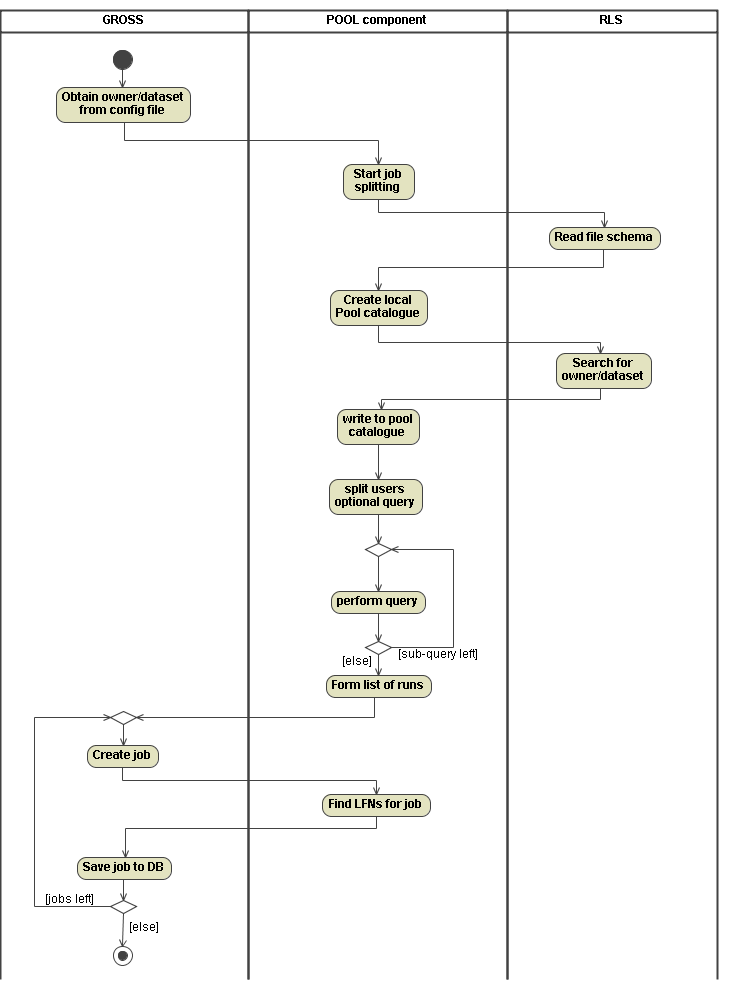
\includegraphics[width=1.\linewidth]{gross/Job_splitting}\\[1mm]
  \caption{Activity diagram showing the task splitting workflow. 
  \label{fig:task_splitting}}
\end{figure}

\subsection{Task splitting}
Each CMS Monte Carlo production job generated a separate run of data, hence it seemed logical to split the analysis task in the same way. This allowed maximum flexibility for job submission. Each job required the minimum number of files for a given number of events and each file was needed by only one job, so allowing each job within a task to be sent to a different site. This splitting was only appropriate for an analysis case where the majority of events were fully analysed, as was the case with most CMS analyses in 2004. This would not be the case with real data where not every event in a dataset would prove interesting to every analysis. Hence this strategy was appropriate for Monte Carlo analyses but not for real data.

The task splitting workflow is illustrated in Figure~\ref{fig:task_splitting}. Once the local file catalogue containing all files within the dataset had been created, a list of runs was produced subject to the optional user-provided metadata query. This list was then used to create the sub-jobs. Once jobs had been configured with their run number they could then obtain a list of their input data files by querying for all of the LFN's for their run. The archive file containing the metadata also had to be discovered and added to the list of input files for each job.

%The number of runs analysed by a job was user configurable as the time taken for anlyses varied greatly. later

Each job was configured with the correct data selection, input and output data files. Files generated during configuration included a POOL XML fragment listing the input data, a JDL file for the RB and a configuration file for the wrapper script that ran the appropriate workflow on the worker node. All information was saved to the database, so in subsequent actions the entire task and all jobs could be recreated without repeating the data discovery or task splitting.

%The user analysis application was run by a wrapper script which also set up the CMS environment and handled output files at the end of the job. Each job required a configuration file to steer the job wrapper, a POOL XML file catalogue fragment listing the input data files and a JDL file describing the job to be given to BOSS. The steering file contained all the information necessary for running the job, i.e. the ORCA version and executable to run. The JDL file for each job contained the list of required input data and the required ORCA version, to allow the RB to steer the job to the correct location.

%Once a task had been split the constituent jobs were saved to the database. All relevant information was saved including the POOL XML fragment - therefore at submission no information had to be re-calculated.

%%%%%
%Step before submission - files etc...
%ave to database
%split acording to directive  - 1 or many runs per job
%job - list of files needed
%steering file
%Pool XML Fragment - only files job needs + meta
%metadata
%out files
%prepare tar - wrapper, BOSS, etc..
%register to BOSS
%unique Suffix i.e. task name
%%%%%

\subsection{Task submission}
To submit a task the user provided the task id and the desired scheduler. GROSS then retrieved the task and sub-jobs and prepared the submission files. These files included the user-defined files, ORCA configuration file, user's executable, user libraries, wrapper script and the wrapper script steering file. Each job was submitted to BOSS with the GROSS job type to activate the specialised monitoring. After submission each job record in the GROSS database was updated to point to the BOSS job record, which contained information such as scheduler id and status.

%bit more about scheduler stuff temp file creation? BOSS etc? BOSS job archive dbUpdator

\subsection{ORCA wrapper script}
%workflow when landing on worker node
%
Before ORCA could be run a number of steps had to be taken: the CMS environment needed to be set, input files  located, the user's executable and libraries prepared and many other operations. In order to perform these tasks a wrapper script was necessary. The script had to be lightweight, fast and capable of running on many different types of operating system and architecture. This script was implemented as a shell script that provided a capable but lightweight solution.

%This script was implemented as a shell script, this was chosen as a capable but lightweight solution. The LCG utilities that provided functionality for RLS and file operations were also required, however these were available by default on LCG worker nodes. An installed version of ORCA complete with POOL file catalogue commands was also needed. 

%A way to extract the metadata from the zip archive was required, however the usual program for this unzip (or gunzip) was not always available on worker nodes. This was solved by using the program responsible for java archives which was also able to extract files from zip archives, and as the LCG tools required java this was always present. 

Once a job began on a worker node a process similar to the job preparation step, but in reverse, was run. The local scheduler system started the BOSS jobExecutor, which had to set its own environment before starting the GROSS wrapper. The GROSS wrapper script then set the local CMS environment before starting ORCA. 
%By the time BOSS started the GROSS wrapper script the monitoring had Been activated and all files brought by BOSS were available. 
%The wrapper script printed checkpointing, information and error messages which were recognised by the customised BOSS monitoring scripts. 

%The standard output and error of the wrapper script were continually monitored by BOSS. The wrapper script provided mechanisms for printing out checkpointing, information, warning and error messages. These messages were available to be picked up by BOSS's monitoring. These messages were printed out regularly by the script so the user could follow the scripts progress. 

The wrapper script obtained its configuration information from the steering file. If the script was unable to locate this file the wrapper aborted. Once located this file was parsed and its contents (key-value pairs) placed into variables within the script. After this a check was performed to confirm that certain critical variables were defined. These variables included executable name, ORCA version etc.

The CMS software area was located using an LCG-defined environment variable. In this area was a script, created by the CMS software installation, that set up the CMS environment. After the CMS environment was available the ORCA environment was required. The GROSS wrapper script took the version of ORCA requested, checked its availability and sourced its environment.

%Next all the required files, both local and grid, had to be checked and properly handled. A temporary area to run ORCA in had been created so the files brought with GROSS had to be moved there. These files included the ORCA configuration file, POOL XML fragment and any other files requested by the user. An environment variable was created pointing at the POOL XML fragment that had the effect of making all subsequent POOL file catalogue commands use this catalogue. 

\begin{figure}[!tb]
  \centering
  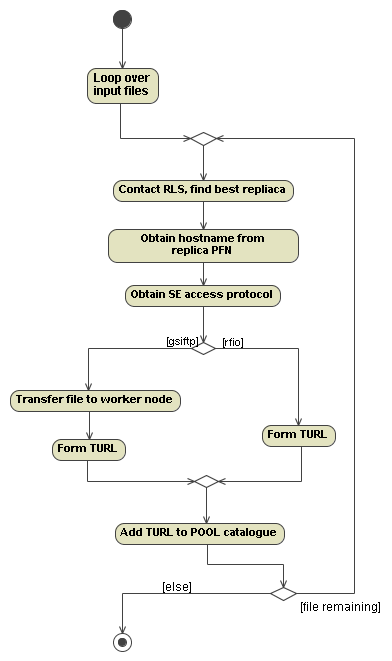
\includegraphics[width=0.55\linewidth]{gross/Wrapper_FileAccess}
  \caption{Activity diagram showing wrapper script workflow for locating input files. The deprecated direct file access protocol is not shown.
  \label{fig:Wrapper_fileAccess}}
\end{figure}

Next the input data files had to be located. It was LCG policy to send jobs only to sites that hosted all of the required files on their SE. The LCG SE supported three file access protocols: direct file access, RFIO and GSIFTP. Direct file access assumed that files were available from the worker node filesystem. This mechanism was deprecated due to scalability issues and was dropped from later LCG releases. RFIO was a widely supported file access mechanism within HEP that allowed files stored on a server to be accessed from remote clients and was the recommended access method. It required that applications support the protocol, which most HEP applications at the time did. The GSIFTP protocol was the standard mechanism for transferring files between LCG SE's. It was an FTP implementation that utilised the LCG security model (X509 certificates). ORCA could not use GSIFTP for file access and so files first had to be downloaded to the local filesystem. This resulted in the use of unnecessary bandwidth between the SE and WN and the need for temporary disk space on the worker node. By definition an LCG SE had to support the GSIFTP protocol whereas the others were optional. This meant that the script had to discover the access protocols provided by the SE and take appropriate action.

A site may have had more than one SE hence, for each file, the hosting SE had to be found and the supported protocols discovered. The workflow is illustrated in Figure~\ref{fig:Wrapper_fileAccess}. This information could be obtained from the brokerInfo file~\cite{citeulike:835506}, a file created by the RB on job matching and sent with the job, containing information about each SE at the site that hosted input data, including supported protocols. Thus for each file the script obtained the location of the closest replica from the RLS including the hosting SE. Using the information in the brokerInfo file the SE's list of supported access protocols was discovered. The scripts then applied rules to find the correct access mechanisms, trying in the order RFIO, file and then GSIFTP. Once the access protocol had been discovered the script had to form a correct contact string, possibly copy the file locally (in the case of GSIFTP) and update the XML POOL fragment, sent with the job, with the new contact string. 
%For each LFN POOL file catalogues allow multiple contact strings and when asked for a contact string provide one of them at random. Therefore all existing contact strings for a LFN were overwritten with the correct value.

Even if the metadata archive was available over RFIO it was copied to the local disk to allow the metadata files to be extracted. 
%. This was because the program used to extract files from the archive could not use the RFIO protocol.
The metadata archive contained several POOL XML fragments describing the metadata files. Once extracted the script merged these with the POOL fragment from GROSS and processed each of the files, setting the contact strings to point to the newly-extracted files. The metadata was virgin, therefore ORCA could not read it and go straight to an event within a data file. A program distributed with ORCA first had to be run on the event data files to find the event collection identifier, which was then added to the ORCA configuration file to allow ORCA to access the events.

Before running the user's executable a check was made to ensure that all of the required libraries were available. If libraries were missing the script exited with an error. ORCA was capable of providing useful output but still exiting with a non zero exit code, in this case the script continued but recorded the exit code for later use. Once an output file was found, it had the optional task name appended and was either saved to an SE and registered with the RLS or returned via the LCG output sandbox. Figure~\ref{fig:Wrapper_OutputFilesRLS} shows the workflow for registering output files with the RLS. Files were saved to an LCG SE local to the the site and registered with the same LFN as their filename.

\begin{figure}[!tbp]
  \centering
  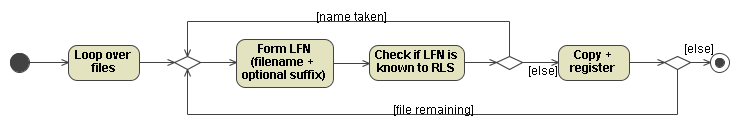
\includegraphics[width=1\linewidth]{gross/Wrapper_OutputFilesRLS}
  \caption{Activity diagram showing wrapper script workflow for registering output files with the RLS. If an LFN already existed GROSS did not overwrite it. It was the user's responsibility to ensure that output from previous tasks with the same optional suffix no longer existed.
  \label{fig:Wrapper_OutputFilesRLS}}
\end{figure}

Finally the script removed all files it had created and exited with the same error code as that of the user's ORCA executable. BOSS recorded the exit code (and various statistics), collected all of the output files and exited. 

\subsection{Querying and output retrieval}
Once the task had been submitted the status of its constituent job's could be queried. If GROSS was unsure of a jobs status, i.e. the job had been submitted but not retrieved, GROSS queried BOSS. BOSS then queried the database for the job state, and, if this could not be determined, the scheduler was queried. 

All GROSS jobs were submitted to BOSS as a member of the GROSS job type. This job type was registered during the GROSS installation and registered monitoring scripts designed to monitor the wrapper error and information messages. If the running job was able to contact the GROSS database then these messages were continually relayed to the database. The database held the last message in each category for each job. This information was accessible from the GROSS command line.

Once a job had finished the output could be retrieved. When a user requested that a task's output be retrieved, GROSS located the jobs that had completed and asked BOSS to retrieve their output files. If the output was retrieved successfully the GROSS database was updated. By using the GROSS client the user could later determine where a particular task's output had been saved.

\subsection{Local farm submission}
Job preparation and execution on a local batch farm required significantly different steps from a grid submission, requiring the introduction of another task type. This task type assumed that the user had a POOL file catalogue containing a locally available dataset. This may have been the RLS in the case where a user wished to bypass the LCG and submit directly to local resources. This only worked in the case where the registered PFNs were also the file contact string, which was the case at CERN but not at LCG sites in general. 
%Though this worked only where the pfns's registered to the RLS were the contact strings for the local site, this was not the case for files saved to LCG SE's but was for CERN. 
The difference in data discovery between the two task types was that the local type resolved file contact strings at creation time whereas grid jobs determined this at runtime given the site at which they ran.

The local version of the wrapper script provided similar functionality to the grid script. File access was simplified as it was assumed that the POOL fragment already had correct contact strings. Not all local batch systems supported input or output file handling, therefore all files had to be available on a shared filesystem. At the end of a job the output was copied back to another location on the shared filesystem specified when the task was created. The GROSS output retrieval step was not necessary.

\section{Performance and useability}
Unfortunately GROSS development progressed more slowly than originally envisaged and DC04 had already begun by the time it was released. Due to the amount of data to be analysed an automated procedure using custom software agents had been developed (Figure~\ref{fig:dc04_analysis}). These agents were tightly coupled with the transfer system. Once files appeared at CERN and were registered in the RLS they were transferred to a remote site, the replica registered and an analysis job sent via LCG. The executables and libraries were sent together with the job and the output was saved to an SE and registered to the RLS. Job submission and monitoring were provided by BOSS. In the last two weeks of DC04 15,000 jobs were sent, with a grid efficiency (i.e. the efficiency for a job to be executed at a site irrespective of the success of the application) of 90-95\% and a latency of 20 minutes between files appearing at CERN and their remote analysis~\cite{citeulike:621630, Fanfani:2004gh}.

\begin{figure}[tbp]
  \centering
  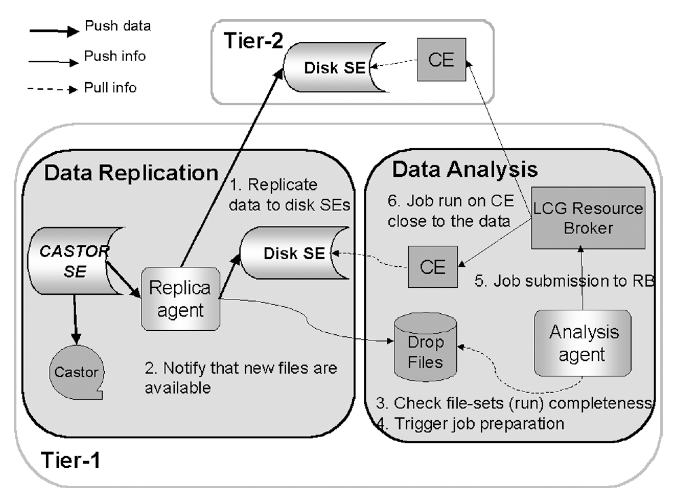
\includegraphics[width=0.85\linewidth]{gross/data_analysis}
  \caption{DC04 real time analysis chain.~\cite{citeulike:621630}
  \label{fig:dc04_analysis}}
\end{figure}

During this time the developers evaluated, tested and made several enhancements and bug fixes to GROSS. While all functionality worked as intended the performance was worse than expected. Specifically the data discovery step was found to be unacceptably slow, which was traced to poor performance of the RLS. 

The RLS consisted of several components: the Local Replica Catalog (LRC), which maintained the list of replicas at a site, the Replica Location Index (RLI), which indexed multiple LRC's and the Replica Metadata Catalog (RMC), which held file metadata~\cite{citeulike:623288}. Within LCG the RLS had only been implemented as a single LRC (and RMC) per experiment instead of per site as it had been designed. The LRC had been evaluated with inserts, deletes and queries on LFN's. These tests and experience during DC04 showed acceptable performance~\cite{citeulike:623294, baud2004eld}. However, metadata tests had only involved inserts and deletes. Once the system was queried for all files meeting certain criteria it became apparent that performance was unacceptable~\cite{citeulike:623294, baud2004eld}. Queries for all files belonging to an average CMS dataset ($~\sim$1000 runs), as required by GROSS, took 2--3 hours to complete~\cite{citeulike:623294}.

The real time analysis was only concerned with LFNs and so was able to avoid the poor performance of the RLS with metadata queries. GROSS, however, was based on the premise that the user did not know the files they wished to analyse, only the dataset. One way to improve performance was to use the POOL file catalog commands manually to perform the search of the RLS and to store the results in an XML catalogue. If this was then used with GROSS and multiple tasks were created against the dataset, performance was seen to improve with data discovery taking minutes rather than hours.

%more on usage?

\section{Post DC04 distributed analysis}
%put 0_2_0 here i.e. intermediate metadata, multiple runs ...

After DC04 CMS decided that instead of requiring LCG to optimise the RLS it would eliminate the need for a global file catalogue. Instead a central catalogue would keep a mapping between datasets and sites. Each site would then host its own file catalogue (possibly more than one). In this model the central catalogue would contain significantly less information and be subject to fewer simpler queries, which improved performance. Each site had a web-accessible service, known as a  PubDB, which would return the correct file catalogue(s) for a dataset~\cite{citeulike:623034}. The file catalogue could be any POOL file catalogue and was generally either XML files or a MySQL database. 

The data movement system was re-engineered but still consisted of transfer agents at each site controlled by a central database. The site agents periodically queried the database and discovered any outstanding data requests. The agents downloaded the relevant files and marked the transfers as complete in the database. Only event data was known to the CMS data management system, hence, before the dataset was available for analysis the metadata had to be downloaded in a separate publishing step. Here the virgin metadata was downloaded from CERN and populated. These and the event data files were then added to the local POOL file catalogue(s).

The result of these changes was that jobs no longer needed to carry their own file catalogue or know \emph{apriori} which files were required. It was the responsibility of the site to provide the job with the means to locate all files needed at runtime.

%%%%%\section{New GROSS architecture}
%%%%%
%This change sped up GROSS considerably and reduced the amount of data stored in the database. When the task is created the only data discovery steps needed are to ensure that the dataset exists and that at least one site has a copy. During the time interval between task creation and submission a site status may have changed so the list of hosting sites was formed at submission time.  GROSS contacted the hosting sites to find the contact strings for their file catalogues. The list of sites is then added to the JDL to allow the RB to send the job to the correct site and the list of file catalogues is provided in the steering file for the wrapper script.
%%%%%

In the transition period between the phasing out of the RLS and adoption of the PubDB system an interim solution was used. Full (i.e. non virgin) metadata was made available via the CMS MC production system. Once a dataset had been produced it was copied to CERN, where the metadata was fully populated with information about all event data. These metadata files were then made available from the CMS web server. During the data discovery stage GROSS contacted both the RLS for event files and the CMS webserver for the metadata and a POOL catalogue fragment. These were then both sent with the jobs. This temporary procedure was only needed while the PubDB system was being developed.

\section{CRAB}
Around this time another tool called CRAB (CMS Remote Analysis Builder)~\cite{citeulike:876380}, developed by a group from Italy, was released. This tool was similar to GROSS with only minor differences. During December 2004 a meeting was held in Bologna to decide the future of CMS distributed analysis. At this meeting a comparison of the two applications was carried out. 

CRAB was written in Python and did not utilise BOSS. These choices and the relatively large development team allowed CRAB to develop PubDB support before GROSS. The lack of BOSS integration simplified the installation of the software and eliminated the requirement for a MySQL database but resulted in poor job tracking and logging. There was no central repository where information about all tasks could be found. Each task had its own directory for submission and output files and this directory had to be retained if the user wished to retain knowledge of the task.

CRAB also had other features aimed at simplifying its use. It was integrated with the CMS build system and thus, with the appropriate ORCA environment set, could locate the users executable and all libraries. GROSS, in contrast, required the full path to each to be listed in the configuration file. With CRAB, tasks could be created, submitted and scheduled for automatic file retrieval with a single command. The same workflow in GROSS required at least three separate commands. However, GROSS had a much clearer and more consistent command line.

Overall it was felt that GROSS provided a more uniform interface and better job monitoring and bookkeeping but CRAB was easier to install and provided many features that simplified the analysis process for the user.

As a result of the meeting it was decided that both applications would continue to be developed whilst an evaluation by the CMS physics community was conducted. CRAB would investigate using BOSS to provide job submission and logging and GROSS would adopt the PubDB system and some of the ideas in CRAB aimed at simplifying and automating the analysis process for the user.

\section{New architecture and features}
Until the meeting in Bologna GROSS had been distributed together with BOSS. Many sites, however, already had an installation of BOSS from CMS MC production activities, so it was decided to package GROSS separately.

The change to using the PubDB system required a large change in the architecture of GROSS. Previously each job had known about all input and output files, but this information was no longer necessary. GROSS now relied on a correct POOL file catalogue at the site to contain the requested data. The facility for users to send jobs using their own POOL file catalogue to local resources was still maintained.

Previously, analysis with GROSS had only focused on the Hits data tier, whereas most advanced Monte Carlo analyses required access to both the Hits and the Digis. This required access to data from two owner/datasets and possibly the pile-up dataset also. The PubDB system had been designed to cope with this and for each owner/dataset the central PubDB listed the related owner/datasets. In the task specification file the user could request data tiers related to the the specified owner/dataset. GROSS would then ask the central PubDB catalogue for their entries as well. Sites were not required to host entire datasets, only a continuous range of complete data runs. For each job GROSS required that a site hold the same run in all data tiers, plus the complete pile-up dataset. The ability to access multiple data tiers was only required for analysis of Monte Carlo data.

The move to PubDB improved performance considerably. The data discovery step was now simplified, when the task was created the only data discovery steps needed were to ensure that the dataset existed and that at least one working site had a copy. This was in contrast to the previous situation where every file within the dataset has to be located. The combination of the new system and simpler queries resulted in a considerable performance gain, with data discovery taking approximately 10\,s.

During the interval between task creation and submission the status of the sites may have changed, so the list of sites was formed at submission time. GROSS contacted each hosting site to find the contact strings for the file catalogues. If a site did not respond within a set time it was skipped and GROSS moved to the next site. The list of appropriate sites was added to the JDL to allow the RB to send the job to the correct site and the list of file catalogues was added to the steering file for the wrapper script.

Previously GROSS had split a task into one job per run. However, as the time required for different analyses varied greatly this was modified so that the user could change this. As well as specifying the number of runs to analyse in a job the user could also specify the start and end run numbers if they did not want to analyse all runs within the dataset.

During Autumn 2004 LCG sites began to migrate their operating systems from RedHat Linux 7 to systems compatible with Scientific Linux CERN 3, SLC3~\cite{SLC3} (a RedHat Enterprise 3 derivative~\cite{RHEL}). Applications built on SLC3 could not run on RedHat 7 systems. LCG sites specified their operating system in the information system. If a user wished to run on a certain architecture they could add a ClassAd requirement to the task specification file, which would then be passed to the RB at submission time. To allow access to all sites GROSS provided the option for users to send their source code and have their analysis application built on the worker node. If this was requested the user's code would be built in an ORCA environment on the worker node, with the resulting executable automatically linking with the standard ORCA libraries already present at the site. If any errors were encountered during compilation the job would abort.

%The task querying functionality in GROSS had lower than expected performance. The cause of this was found to be due to the handling of status queries within BOSS's LCG scheduler script. Rather than performing a simple status query on each job, the plugin requested the status of all BOSS jobs submitted via LCG and then searched amongst this list for the status of the particular job. This problem only became evident with time as more and more jobs had been submitted. This was compounded as BOSS had no knowledge of the task structure and therefore queries of a tasks status resulted in a separate status query for each job, each of which queried all jobs submitted via LCG. As GROSS was now packaged separately from BOSS and sites all had their own version's it was not possible to patch the LCG query script. Therefore a temporary fix was introduced to GROSS, it was impossible to speed up BOSS's query so instead the approach was to minimise the number of times the query was run. Oringinally for each job a separate BOSS command was run that returned the status of that job, this was changed to a query that returned the status of all jobs submitted via LCG, these results were then cached locally by GROSS. When the status of the next job in the task was requested GROSS looked in this hash table to check for a match, if found this was returned if not the BOSS query was executed as usual. This sped up the query considerably, especially for large tasks.

During one of the LCG upgrades, limits on the input and output sandbox sizes were introduced. The RB stored these and a number of users were sending and/or retrieving very large files via them. This had the effect of filling up the RB's disk and affecting its performance. The limit imposed on input sandboxes was 10MB. GROSS sent the user's pre-compiled binaries as well as files needed by both GROSS and BOSS. The ClassAd library, which was sent to allow BOSS to read its configuration file, was about 7MB, which, together with the user's executable, easily exceeded this limit. It would have been possible to install the ClassAd library at each site, thus circumventing the restriction. However this would require support for each site along with a versioning mechanism to handle different BOSS versions. Thus it was decided that the BOSS developers should attempt to reduce the size of the libraries required by BOSS. A simpler version of ClassAds, called ClassAdLite, was developed which was only a few hundred kB.

In order to help reduce the output sandbox size the facility to allow files to be saved to a set path on a SE of the user's choice, without being registered with the RLS, was introduced. This was easier for users to use than the RLS as they could see files accumulate on an SE, e.g. their private area on CASTOR at CERN, rather than having to query a remote service.

Originally it was foreseen that automatic output retrieval would be handled by a cron-like entity calling GROSS at regular intervals to download any remaining output files. However, the availability of cron was not guaranteed at every site from which users submitted CMS jobs. An alternative method was chosen that made use of an agent process to periodically run GROSS. If, when the user submitted a task, they requested this functionality the script was started on the UI after submission. This script slept for a user-configurable time, then woke and ran GROSS telling it to retrieve any available output for the task. If no output was available the script would go back to sleep. When GROSS reported that all output had been collected the script would exit and if the script was still active after a user-configurable time limit (by default 2 days) it would exit anyway. This was to prevent it from running forever when a problem prevented retrieval of the output. The script wrote to a log file so that users could follow its progress and see how much output remained. If the user ended the session on that machine the process would continue, as it ignored SIGHUP signals. This feature was not enabled by default due to concerns about users starting large numbers of processes on popular machines. 

Output files were stored in a separate directory for each job under the user-specified area, with the optional user suffix appended to each file. As a result of the task splitting it was not uncommon for a user to have hundreds of small ROOT files in different directories. This made keeping track of files or running ROOT over the files inconvenient. Therefore new functionality was introduced that allowed the user to obtain one root file for a whole task. 

By running a script in the GROSS distribution the user could merge all the ROOT files within a task. It was also possible for the user to merge only the output from a subset of the jobs in the task. This script ran GROSS to discover the location of the output files, and any jobs that had finished but whose output had not been retrieved had their output collected. A search for ROOT files was then carried out and any found were added to the list of files to be merged. ROOT was then run, merging all the input files to create a new ROOT file in the specified location.

With jobs submitted to the LCG it was not uncommon for a number in any given task to suffer transient errors, either within the LCG workload management system or because of the configuration of an individual site. To help with this problem a mechanism for resubmission of failed jobs was added. Using this command GROSS would resubmit any failed jobs in a task, or job range within a task. 

Real time monitoring was improved by modifying the GROSS job type to recognise the standard ORCA event number printout. This allowed users to monitor the current progress of their jobs.

%multiple out files
%gross split run - crab events
%merge with BOSS
%Meeting december ??
%decided 
%  1 step submission
%  laptop - prepare online - simpler?
%  move to pubdb - timeout automate etc...
%  need ancestor datasets
%  scram integration
%  auto retrieve
%  non virgin metadata
%class as lite 
%crab?? what mention?
%scram build

\section{Community Evaluation}
Once most of these changes had been made GROSS was made available to the CMS physics community. GROSS was evaluated by members, including the convenor, of the Higgs PRS (Physics Reconstruction and Selection) analysis group. GROSS was used to perform analysis for $\tau$ jet studies and Higgs searches on Monte Carlo data.

The $\tau$ studies consisted of two areas of activity: jet calibration and HLT studies. The calibration study involved developing a Monte Carlo jet \ET calibration for $\tau$ jets. This was achieved by running over a sample of 100,000 hadronically decaying $\tau$'s and comparing the Monte Carlo and reconstructed jet \ET. An algorithm was then developed in ROOT to relate the two. The HLT $\tau$ jet studies looked at trigger optimisation specifically for the MSSM heavy Higgs decaying to two $\tau$ jets.

Higgs analyses included the channels MSSM $H \rightarrow 2 \tau $ jets, MSSM $H \rightarrow 2 \tau \rightarrow \tau \textrm{jet} + l$, MSSM $H \rightarrow 2 \tau \rightarrow 2l$ and MSSM $H^{+} \rightarrow \tau$. These analyses involved running over both signal and background datasets. Backgrounds included QCD multi-jets, W$ + $jets and Z/$\gamma \rightarrow \tau \tau$. The analysis of signal events required the full analysis of the majority of events. Where the backgrounds were likely to be rejected they were preselected, during generation, to be more likely to pass the analysis cuts. Thus this testing used the majority of the available sample and hence did not represent a realistic indicator of performance with real data. 

In these analyses 4 users created $\sim$220 tasks analysing 22 datasets. A total of 4,381 jobs were submitted to BOSS, of which 4,181 were successfully submitted to a scheduler. Of these 3,134 were submitted to LCG and 1,047 to resources local to CERN. 3,726 jobs finished successfully, representing a success rate of 89.1$\%$ and leaving 455 jobs that exited with errors. These errors generally indicated a problem with the user's code (possibly something that was not apparent during limited use) or a (transient) problem at a site, often with file access. It was not possible to give a detailed breakdown of the various failure modes as the ORCA exit codes did not always correspond to the actual error. Also, any user requested job resubmission would have overwritten the details of the previous job in the database. Thus the 89.1$\%$ success rate represented the rate allowing for re-tries. In total these jobs used over 605 days of computational time.

These statistics were taken from the GROSS/BOSS database. If a running job was unable to contact the database the records may be incomplete. In this case GROSS attempted to correct the situation at the output retrieval stage by running BOSS with the retrieved journal file. This process was not, however, always reliable.

%%%%%%%%%%%%%%%%%%%%%%%%%
%4 users
%13775 jobs
%222 tasks 
%avg 55 jobs per task.
%me - tau calibration, 	bt04_double_tau_hadr, jm03b_qcd_50_80
%slehti MssmA2tau2l	hg03_h2tau_2l_200 hg03_hsm120_mumu hg03_zg80_100_2tau_2l
%Sasha - MssmA2tau2j, 
%        tau HLT 	bt03_mssm_h2tau_jj200 bt03_mssm_h2tau_jj500 bt03_qcd80-120_2tauj jm03b_qcd_50_80
%kinnunen - MssmHighmHchTauJ	hg03_thplus200_tau
%22 datasets
%
%Feedback - merge root files, take all info from db
%           concurrency problems database, 
%           error testing check for edg tools and proxy
%           lsf queue
%           first/last run - easier than meta query (did this apply to pubdb - no)
%           resubmission of failed jobs
%           globus-url-copy out files - not save LFN i.e. to own castor area
%need parent datasets
%prob monitoring - mysql - try to get journal files - not always work          
%%%%%%%%%%%%%%%%%%%%%%%%%

\section{Conclusion}
GROSS met all of the requirements set out in the design phase and was a proof-of-principle tool for distributed analysis within HEP. It proved useful for physicists during work leading up to the writing of the CMS physics TDR~\cite{CMS_TDR_PHYS_vol1}. It allowed a physicist to perform an analysis over large amounts of data distributed between CMS' resources worldwide. The use of GROSS by physicists in their work provided much needed-feedback and allowed the introduction of a large number of bug fixes and new features. 

Compared to CRAB it was felt that GROSS provided better logging and monitoring, implemented through BOSS, but that CRAB was a more lightweight and flexible design. CMS decided that CRAB provided the more appropriate client-facing application, but recognised that GROSS was more robust and through BOSS provided many useful features. Thus it was decided to introduce many of the features GROSS provided, i.e. the task concept and handling, into BOSS, while CRAB would act as a CMS-specific application relying on BOSS to provide the task submission and logging functionality. The BOSS development work is described in the next chapter.
